\documentclass{article}
\usepackage[utf8]{inputenc}
\usepackage{siunitx}
\usepackage{graphics}
\usepackage[american,siunitx]{circuitikz}
\usepackage{amsmath}
\usepackage{svg}
\usepackage{booktabs}
\usepackage{float}
\usepackage{xparse, xfp}
\usepackage{graphicx} 
%\renewcommand{\thesubsection}{\thesection.\alph{subsection}}
\newcommand{\equal}{=}
\ExplSyntaxOn
\NewDocumentCommand{\defcon}{mm}
 {
  \cs_new:Npx #1 { \fp_eval:n { #2 } }
 }
\ExplSyntaxOff

\title{ECE2101L\\Electrical Circuit Analysis II Laboratory\\\,\\Lab 5\\Complete Response of Series RLC Circuits\\\,\\Report\\}
\author{Choi Tim Antony Yung\\\,\\Willis Nguyen\\Phineas Cozmiuc}
\date{2 March 2020}

\begin{document}

\clearpage\maketitle
\thispagestyle{empty}

\newpage
\setcounter{page}{1}

\section*{Objective}
The purpose of this experiment is to explore the behavior of a second order series RLC circuit with Simulink Simscape Power System Toolbox.

\section{Underdamped series RLC circuit}
\begin{figure}[H]
    \centering
        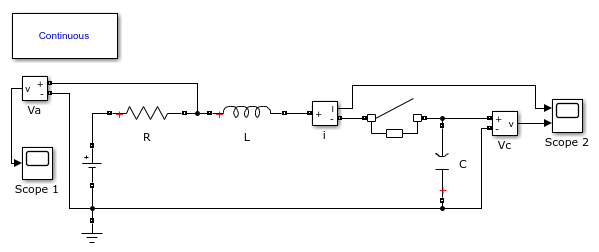
\includegraphics[scale=0.75]{simulink1.png}
\end{figure}

\section*{Procedure}
The above circuit was built as a Simulink model using components from Simulink Simscape Specialized Power System. The ode23t solver was used. The voltage of the DC voltage source was set to \SI{20}{\volt}, inductance was set to \SI{1}{\henry}, resistance was set to \SI{10}{\ohm}, and the capacitance was set to \SI{3000}{\micro\farad}. Switching time of the circuit breaker was set to [0.5 2.5]. Initial capacitor voltage was set to \SI{0}{\volt}

\section*{Analysis}
As the breaker closes, current increases as capacitor and inductor charges. As current increase, the inductor voltage increases in the opposite direction of the current in a passive component, in other words, there is a voltage rise in the direction of the current. Therefore, the upward oscillating value of voltage across capacitor, as it charges at first, have a value larger than \SI{20}{\volt} supplied by the voltage source. As $V_c$ reaches to its maximum value, however, the current changes its direction and decreases the voltage difference between the two terminal of capacitor, and therefore result in a drop of $V_c$. Eventually as the circuit stabilizes and both reactive passive component fully charges, and the inductor act as a short and capacitor act as an open, and therefore no current is flowing through, which deactivates the resistor, the voltage at node Vc is the same as the voltage at node Va, which is the voltage of the voltage source.

\section*{Result}
\begin{figure}[H]
    \centering
        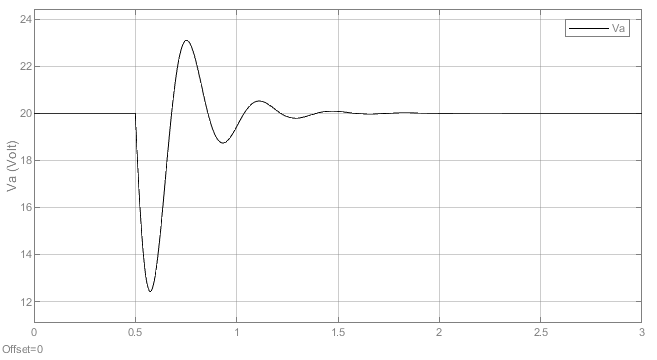
\includegraphics[scale=0.65]{1_Va.png}
\end{figure}
\begin{figure}[H]
    \centering
        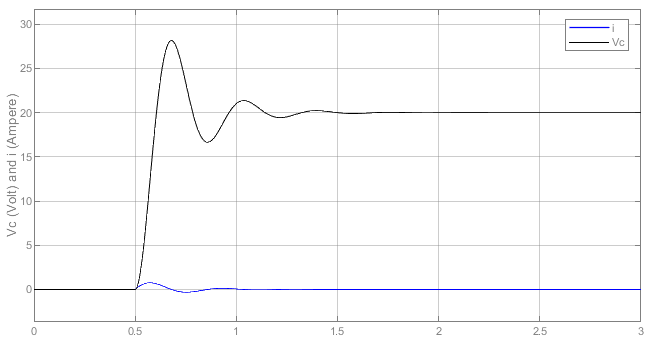
\includegraphics[scale=0.65]{1_Vc_i.png}
\end{figure}
\begin{table}[H]
    \centering
    \begin{tabular}{rrrrr}
        \toprule
        &Initial & Max Oscillating & Max Oscillating & Final\\
        && Upward&  Downward & \\
        \midrule
        Va & \SI{20}{\volt} & \SI{10.67}{\volt} & \SI{7.575}{\volt} & \SI{20}{\volt} \\
        Vc & \SI{0}{\volt} & \SI{28.17}{\volt} & \SI{11.51}{\volt} & \SI{20}{\volt} \\
        I & \SI{0}{\ampere} & \SI{0.7575}{\ampere} & \SI{1.067}{\ampere} & \SI{0}{\ampere} \\
        \bottomrule
    \end{tabular} 
\end{table}

\section{Critically damped and overdamped second order series RLC circuit}

\section*{Theory}
The condition for solution in underdamped, critically damped, and overdamped case in terms of $\alpha$ and $\omega_0$ is the following:
\[ \begin{cases} 
      \alpha < \omega_0 & underdamped \\
      \alpha = \omega_0 & critically\; damped \\
      \alpha > \omega_0 & overdamped 
   \end{cases}
\]
Substituting $\alpha = \frac{R}{2L}$ and $\omega_0 = \sqrt{\frac{1}{LC}}$:
\[ \begin{cases} 
      \frac{R}{2L} < \sqrt{\frac{1}{LC}} & underdamped \\
      \frac{R}{2L} = \sqrt{\frac{1}{LC}} & critically\; damped \\
      \frac{R}{2L} > \sqrt{\frac{1}{LC}} & overdamped 
   \end{cases}
\]
Solving for R:
\[ \begin{cases} 
      R < 2\sqrt{\frac{L}{C}} & underdamped \\
      R = 2\sqrt{\frac{L}{C}}=2\sqrt{\frac{1}{3000\times10^{-6}}}\approx36.515 & critically\; damped \\
      R > 2\sqrt{\frac{L}{C}} & overdamped 
   \end{cases}
\]
Therefore, the circuit will be critically damped with a resistance of $R_{CD} \approx \SI{36.515}{\ohm}$ and overdamped with resistance of $R_{OD} = 100 > \SI{36.515}{\ohm}$
\section*{Analysis}
In the underdamped case, Va oscillates and have a maximum oscillating value lower than the two other cases, in the overdamped case, Va dipped to a much lower value than the two other cases. As the resistor act as a current limiter in this circuit, the change in current is lower when the resistance is higher, which corresponds directly to the voltage of the inductor and capacitor as the voltage of the inductor depends on the rate of change of the current and the voltage of the capacitor depends on the voltage of the inductor. Therefore, voltage across the inductor and capacitor is lower as resistance increases in the critically damped and overdamped case. The oscillation in the underdamped case is also a result of the lower resistance that allows for a much wider swing of current.

\newpage
\section*{Result}
\begin{figure}[H]
    \centering
        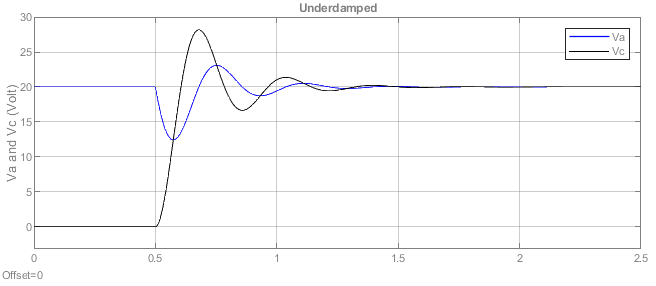
\includegraphics[scale=0.65]{2_UD.png}
\end{figure}
\begin{figure}[H]
    \centering
        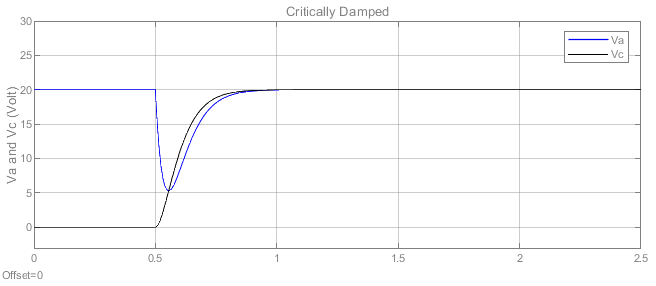
\includegraphics[scale=0.65]{2_CD.png}
\end{figure}
\begin{figure}[H]
    \centering
        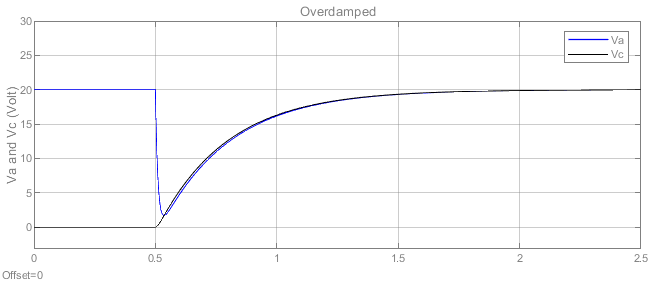
\includegraphics[scale=0.65]{2_OD.png}
\end{figure}

\section{Impact of resistance R on circuit response}
\begin{figure}[H]
    \centering
        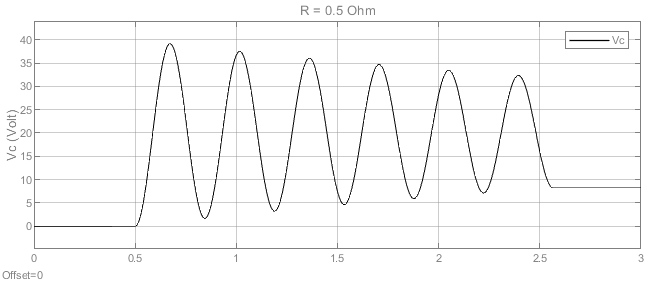
\includegraphics[scale=0.6]{3_0.5.png}
\end{figure}
\begin{figure}[H]
    \centering
        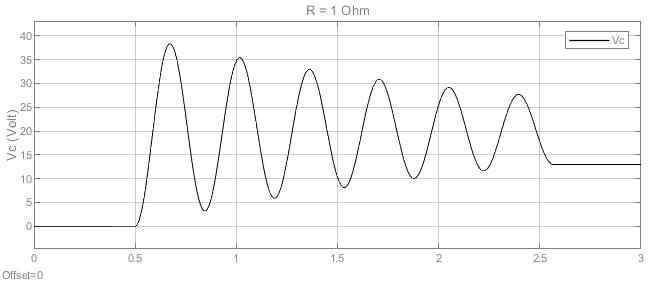
\includegraphics[scale=0.6]{3_1.png}
\end{figure}
\begin{figure}[H]
    \centering
        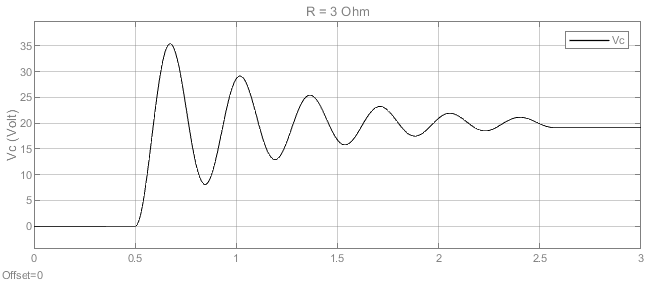
\includegraphics[scale=0.6]{3_3.png}
\end{figure}
As resistance increases, current value was limited to a smaller range and, thus, have a smaller changes and the changes to the voltage of the inductor and therefore capacitor is more limited. Mathematically, this is represented by that the envelop function $e^{-\alpha t} = e^{-\frac{R}{2L}t}$ decays faster as resistance increases.

\end{document}